\documentclass[dvipdfmx]{ujarticle}
\usepackage{eee}

\begin{document}
\title{令和3年 電磁気学II}
\date{}
\author{大山主朗}

\maketitle

\section*{令和3年 電磁気学II 前期中間試験}
\section{以下の(a)及び(d)に示す物理定数は電磁気学を修めた者であれば常識的に覚えていなければならない数値である.それぞれの値を示せ.}
\begin{enumerate}[(a)]
	\item 真空の誘電率$\varepsilon_{0}:8.854 \times 10^{-12}\,\rm{F/m}$
	\item 真空の透磁率$\mu_{0}:1.257 \times 10^{-6}\,\rm{H/m}$
	\item 電子の電荷$e:-1.602 \times 10^{-19}\,\rm{C}$
	\item 電子の静止質量$m:9.109\times 10^{-31}\,\rm{kg}$
\end{enumerate}

\section{$xy$直交座標系において,同量異符号の点磁荷$\pm m$が距離$l$に固定された磁気双極子が存在する.このとき以下の問いに答えよ.ただし,$x$ 方向の基準ベクトルを$\boldsymbol{i}$,$y$方向の基準ベクトルを$\boldsymbol{j}$とする}
\begin{enumerate}[(a)]
	\item 点Aに存在する磁荷$-m$が点P$(x_0,y_0)$に作る磁界$\boldsymbol{H}_{1}$を求めよ.
	\begin{align*}
		\boldsymbol{H}_{1}&=\frac{1}{4\pi \mu_{0}}\frac{-m}{\left(\left(x_0+a\right)^{2}+y_{0}^{2}\right)^{3/2}} \left\{ \left(x_{0}+a\right)\boldsymbol{i}+y_{0}\boldsymbol{j}\right\}\,[\rm{A/m}]
	\end{align*}
	\item 点Bに存在する磁荷$+m$が点P$(x_0,y_0)$に作る磁界$\boldsymbol{H}_{2}$を求めよ.
	\begin{align*}
		\boldsymbol{H}_{2}&=\frac{1}{4\pi \mu_{0}}\frac{m}{\left(\left(x_{0}-a\right)^{2}+y^{2}\right)^{3/2}} \left\{ \left(x_{0}-a\right)\boldsymbol{i}+y_{0}\boldsymbol{j}\right\}\,[\rm{A/m}]
	\end{align*}
	\item 点Pでの磁界$\boldsymbol{H}$を求めよ.
	\begin{align*}
		\boldsymbol{H}&=\boldsymbol{H}_{1}+\boldsymbol{H}_{2}\\
		&=\frac{m}{4\pi \mu_{0}}\left[\frac{-1}{\left(\left(x_{0}+a\right)^{2}+y_{0}^{2}\right)^{3/2}} \left\{ \left(x_{0}+a\right)\boldsymbol{i}+y_{0}\boldsymbol{j}\right\}+\frac{1}{\left(\left(x_{0}-a\right)^{2}+y_{0}^{2}\right)^{3/2}} \left\{ \left(x_{0}-a\right)\boldsymbol{i}+y_{0}\boldsymbol{j}\right\}\right]\,[\rm{A/m}]
	\end{align*}
	\item 磁気双極子モーメント$\boldsymbol{M}$を求めよ.
	\begin{align*}
		\boldsymbol{M}&=m\boldsymbol{l}\\
		&=2am\boldsymbol{i}\,[\rm{Wb\cdot m}]
	\end{align*}
	\item 点Pが原点Oより十分遠方にあると仮定すると,$\sqrt{(x-a)^{2}+y^{2}}\simeq \sqrt{x^{2}+y^{2}}$及び$\sqrt{(x+a)^{2}+y^{2}}\simeq \sqrt{x^{2}+y^{2}}$と近似できる.このことを用いて(c)にて得た磁界$\boldsymbol{H}$を簡略化せよ.
	\begin{align*}
		\boldsymbol{H}&\simeq -\frac{1}{4\pi \mu_{0}}\frac{2am}{\left(x_{0}^{2}+y_{0}^{2}\right)^{3/2}} \boldsymbol{i}\,[\rm{A/m}]\\
		&\left(\simeq -\frac{\boldsymbol{M}}{4\pi \mu_{0}r^{3}}\,[\rm{A/m}]\right)
	\end{align*}
	\item $y$方向に一様な磁界$\boldsymbol{H}_{0}$が存在するとき,磁気双極子にはたらく力のモーメント$N$を求めよ.
	\begin{align*}
		\boldsymbol{T}&=\boldsymbol{M}H_{0}\sin \theta \\
		&=2am\boldsymbol{i}\sin \frac{\pi}{2}\\
		&=2am\boldsymbol{i}\\
		|\boldsymbol{T}|&=2am\,[\rm{Wb\cdot m}],x軸右方向
	\end{align*}
\end{enumerate}

\section{$xyz$直交座標空間において,$xy$平面内に原点Oを中心とする半径$a$の円形ループ電流$I$が流れており,$z$軸上に点P$(0, 0, h)$がある.このとき,点Pに発生する磁界$\boldsymbol{H}$を求めよ.}
\begin{align*}
	ビオ・サバール&の法則を適用する.\\
	y>0に円周上の&微小磁界d\boldsymbol{H}_{1}を\\
	y<0に円周上の&微小磁界d\boldsymbol{H}_{2}を考える.\\
	またそれぞれの&線素ベクトルをd\boldsymbol{l}ととる.\\
	ここで,d\boldsymbol{H}_{1}とd\boldsymbol{H}_{2}の外積より,&2つの磁界は打ち消される方向となっているため,\\
	d\boldsymbol{H}_{1}とd\boldsymbol{H}_{2}を合成した&磁界をd\boldsymbol{H}とする.(\phi:d\boldsymbol{H}_{2}とd\boldsymbol{H}のなす角)\\
	|d\boldsymbol{H}_{1}|=|d\boldsymbol{H}_{2}|&=\frac{Idl}{4\pi r^{2}}\sin \theta\\
	&=\frac{Idl}{4\pi (a^{2}+h^{2})}\\
	d\boldsymbol{H}&=2d\boldsymbol{H}_{1}\cos \phi\\
	&=2d\boldsymbol{H}_{1}\frac{a}{r}\\
	&=2d\boldsymbol{H}_{1}\frac{a}{\sqrt{a^{2}+h^{2}}}\\
	|d\boldsymbol{H}|&=2|d\boldsymbol{H}_{1}|\frac{a}{\sqrt{a^{2}+h^{2}}}\\
	&=\frac{aIdl}{2\pi (a^{2}+h^{2})^{3/2}}\\
	\boldsymbol{H}&=\oint d\boldsymbol{H}_{1}\\
	|\boldsymbol{H}|&=\frac{1}{2}\oint|d\boldsymbol{H}|\\
	&=\frac{1}{2}\oint \frac{aIdl}{2\pi (a^{2}+h^{2})^{3/2}}\\
	&=\frac{1}{2}\cdot \frac{aI}{2\pi (a^{2}+h^{2})^{3/2}} \cdot 2\pi a\\
	&=\frac{a^{2}I}{2 (a^{2}+h^{2})^{3/2}}\,[\rm{A/m}]\quad 上向き\\
	\boldsymbol{H}&=\frac{a^{2}I}{2(a^{2}+h^{2})^{3/2}}\boldsymbol{k}\,[\rm{A/m}]
\end{align*}

\section{$xyz$直角座標空間において,$y$軸上の点$\rm{A}(0, c_{1}, 0)$から点$\rm{B}(0, c_{2}, 0)$まで$y$軸に沿って直線状に流れる電流$I$がある.このとき,$x$軸上の点$\rm{P}(a, 0, 0)$に発生する磁界$\boldsymbol{H}$を求めよ.また,電流$I$の始点Aと終点Bの座標がそれぞれ$(0, -\infty, 0), (0, \infty, 0)$となった場合の点$\rm{P}$に発生する磁界$\boldsymbol{H}$を求めよ.}
	\begin{align*}
	x方向,y方向,z方向の&基底ベクトルをそれぞれ\boldsymbol{i},\boldsymbol{j},\boldsymbol{k}とする\\
	この時&d\boldsymbol{l}=dy\boldsymbol{i}, \boldsymbol{r}=a\boldsymbol{i}-y\boldsymbol{j}\\
	d\boldsymbol{l}\times \boldsymbol{r}&=
	\begin{vmatrix}
	\boldsymbol{i} & \boldsymbol{j} & \boldsymbol{k}\\
	0 &dy & 0\\
	a & -y &0
	\end{vmatrix}
	=dy
	\begin{vmatrix}
	\boldsymbol{i}  & \boldsymbol{k}\\
	a & 0
	\end{vmatrix}
	=-ady\boldsymbol{k}\\
	\boldsymbol{H}&=\int_{C} d\boldsymbol{H}\\
	&=-\int_{C} \frac{aI\boldsymbol{k}}{4\pi(a^{2}+y^{2})^{3/2}}dy\\
	&=-\int_{c_{1}}^{c_{2}} \frac{aI\boldsymbol{k}}{4\pi(a^{2}+y^{2})^{3/2}}dy\\
	h&=a\tan \theta と置換する.\\
	\frac{dh}{d\theta}&=\frac{a}{\cos ^{2}\theta } \quad \therefore dh=\frac{a}{\cos ^{2}\theta }d\theta \\
	また積分範囲は&c_{1}\to c_{2}から\alpha-\frac{\pi}{2} \to \beta -\frac{\pi}{2}に変更される.\\
	&=-\int_{\alpha-\frac{\pi}{2}}^{\beta -\frac{\pi}{2}} \frac{a^{2}I}{4\pi a^{3}(1+\tan^{2}\theta)^{3/2}}\boldsymbol{k^{}} \frac{a}{\cos ^{2}\theta }d\theta\\
	&=-\frac{I}{4\pi} \boldsymbol{k} \int_{\alpha-\frac{\pi}{2}}^{\beta -\frac{\pi}{2}} \frac{1}{(1+\tan^{2}\theta)^{3/2}} \frac{1}{\cos ^{2}\theta }d\theta\\
	&=-\frac{I}{4\pi a} \boldsymbol{k} \int_{\alpha-\frac{\pi}{2}}^{\beta -\frac{\pi}{2}} \frac{1}{(\frac{1}{\cos^{2} \theta })^{3/2}} \frac{1}{\cos ^{2}\theta }d\theta\\
	&=-\frac{I}{4\pi a} \boldsymbol{k} \int_{\alpha-\frac{\pi}{2}}^{\beta -\frac{\pi}{2}} \cos \theta d \theta \\\
	&=-\frac{I}{4\pi a} \boldsymbol{k} \left[\sin \theta  \right]_{\alpha-\frac{\pi}{2}}^{\beta -\frac{\pi}{2}}\\
	&=-\frac{I}{4\pi a} \left\{\sin \left(\beta -\frac{\pi}{2}\right) -\sin \left(\alpha-\frac{\pi}{2}\right) \right\}\boldsymbol{k}\\
	&=-\frac{I}{4\pi a} \left(-\cos \beta +\cos \alpha \right)\boldsymbol{k}\\
	&=-\frac{I}{4\pi a} \left(\cos \alpha -\cos \beta \right)\boldsymbol{k}\,[\rm{A/m}]\\
	始点Aと終点B&の座標がそれぞれ(0, -\infty, 0), (0, \infty, 0)の場合は\\
	\alpha=0, &\beta =\pi であるので\\
	\boldsymbol{H}&=-\frac{I}{4\pi a}\cdot 2 \boldsymbol{k}\\
	&=-\frac{I}{2\pi a} \boldsymbol{k}\,[\rm{A/m}]
	\end{align*}


\section{半径$a$の半円と半径$b$の半円が接続された導体に電流$I$が流れている.このとき,半円の中心Oに発生する磁界$\boldsymbol{H}$を求めよ.}
	\begin{align*}
	x方向,y方向,z方向の基底ベクトル&をそれぞれ\boldsymbol{i},\boldsymbol{j},\boldsymbol{k}とする\\
	半径aの半円電流がつくる微小磁束,&磁束をそれぞれd\boldsymbol{H}_{a}, \boldsymbol{H}_{a}とする\\
	|\boldsymbol{H}_{a}|&=\oint |d\boldsymbol{H}_{a}|\\
	&=\frac{I}{4\pi r^{2}}\sin \frac{\pi}{2} \oint dl\\
	&=\frac{I}{4\pi r^{2}}\pi r\\
	&=\frac{I}{4r}\,[\rm{A/m}]\\
	d\boldsymbol{l}\times \boldsymbol{r}&より \\
	\boldsymbol{H}_{a}&=-\frac{I}{4a}\boldsymbol{k}\,[\rm{A/m}]\\
	半径bの半円電流がつくる&磁束を\boldsymbol{H}_{b}とする\\
	d\boldsymbol{l}\times \boldsymbol{r}&より \\
	\boldsymbol{H}_{b}&=\frac{I}{4b}\boldsymbol{k}\,[\rm{A/m}]\\
	\boldsymbol{H}&=\boldsymbol{H}_{a}+\boldsymbol{H}_{b}\\
	&=\frac{I}{4}\left(\frac{1}{b}-\frac{1}{a}\right)\boldsymbol{k}\\
	b&>aより\\
	&=-\frac{I}{4}\left(\frac{1}{a}-\frac{1}{b}\right)\boldsymbol{k}\,[\rm{A/m}]
	\end{align*}

\section{$xyz$直交座標系においてTVアニメ版だと「第5使徒ラミエル」,新劇場版だと「第6の使徒」と呼ばれるような$(\pm a, 0, 0), (0, \pm a , 0), (0, 0, \pm a)$の点を通る正八面体がある.この正八面体の各辺に図のように電流$I$が流れている.このとき,原点Oに発生する磁界$\boldsymbol{H}$を求めよ.}
	\begin{align*}
	x方向,y方向,z方向の基底ベクトル&をそれぞれ\boldsymbol{i},\boldsymbol{j},\boldsymbol{k}とする\\
	まずx-y平面について考える&\\
	各辺が原点Oにつくる&磁界それぞれ,打ち消し合うため\\
	\boldsymbol{H}_{xy}&=0\,[\rm{A/m}]\\
	次にy-z平面について考える&\\
	同様に各辺が原点Oにつくる&磁界それぞれ,打ち消し合うため\\
	\boldsymbol{H}_{yz}&=0\,[\rm{A/m}]\\
	次にx-z平面について考える&\\
	同様に各辺が原点Oにつくる&磁界それぞれ,打ち消し合うため\\
	\boldsymbol{H}_{xz}&=0\,[\rm{A/m}]\\
	\boldsymbol{H}&=\boldsymbol{H}_{xy}+\boldsymbol{H}_{yz}+\boldsymbol{H}_{xz}\\
	&=0\,[\rm{A/m}]
	\end{align*}

\section{磁化されていない強磁性体に磁界$H$を外部から印加し,強磁性体内部での磁束密度$B$を観測すると,図3に示すような結果が得られた.このとき,図中の行程1:点$\rm{O}\to$点$\rm{P_{1}}$,行程 2:点$\rm{P_{1}}\to$点$\rm{P_{2}}$,行程3:点$\rm{P_{2}}\to$点$\rm{P_{3}}$,行程4:点$\rm{P_{3}}\to$点P4,行程5:点P4 $\to$点$\rm{P_{5}}$, 行程6:点$\rm{P_{5}}\to$点P6,行程7:点$\rm{P_{6}}\to$点P1の7つの行程に着目して,測定結果を説明せよ.}
$B-H$曲線が直線にならない理由は,磁気分子間の摩擦があるため,その磁化の状態を保とうとする抵抗があるからである.そのため,はじめ磁化されていない鉄は,その現状を維持しようとするため磁化が進みにくい.
しかし,一旦磁化された鉄は,その磁化を維持しようとするため,磁界を減少させても,磁界の強さに応じた経路を辿らず,以前の磁束密度には減少しない.すなわち,強磁性体には以前の磁化の経路によって異なる特性を示す.このような現象を磁化特性のヒステリシス現象という.

以下に行程について説明する.

最初に磁化するときには磁化の強さ$H$を強くしていくと,磁束密度$B$は行程1の経路を通る.
磁束密度が点$P_1$に達したとき,今度$H$を減少させていくと,$B$は元の行程1を通過せずに,新しい行程2に沿って減少していく.このとき,$H$が$0$になっても$B$は$0$にならずに$P_2$だけ残る.この$P_2$を残留磁束密度という.

\clearpage
\setcounter{section}{0}
\section*{令和3年 電磁気学II 前期期末試験}
\section{以下に示す物理定数は電磁気学を修めた者であれば常識的に覚えていなければならない数値です.それぞれの値を示していただければ幸いです.よろしくお願い申し上げます.}
\begin{enumerate}[(a)]
	\item 電子の電荷$e:-1.602 \times 10^{-19}\,\rm{C}$
	\item 真空の誘電率$\varepsilon_{0}:8.854 \times 10^{-12}\,\rm{F/m}$
	\item 真空の透磁率$\mu_{0}:1.257 \times 10^{-6}\,\rm{H/m}$
	\item 電子の静止質量$m:9.109\times 10^{-31}\,\rm{kg}$
\end{enumerate}

\section{昔々あるところに\wfig{1}に示すような,断面が半径$a$の円柱状の内導体と,内径$b$,外径$c$の厚みのある円筒状の外導体を有する無限長同軸ケーブルありました.この同軸ケーブルは内導体と外導体はそれぞれの中心軸を共有するように配置されています.どこからともなく,内導体に一様な電流$I$が,外導体に内導体とは逆方向に一様な電流$I$が流れています.内外導体の中心軸に垂直な平面内における中心軸からの距離を$r$としたとき,同軸ケーブルの周囲に発生する磁界$H$を導出してみましょう.}

\begin{figure}[h]
	\centering
	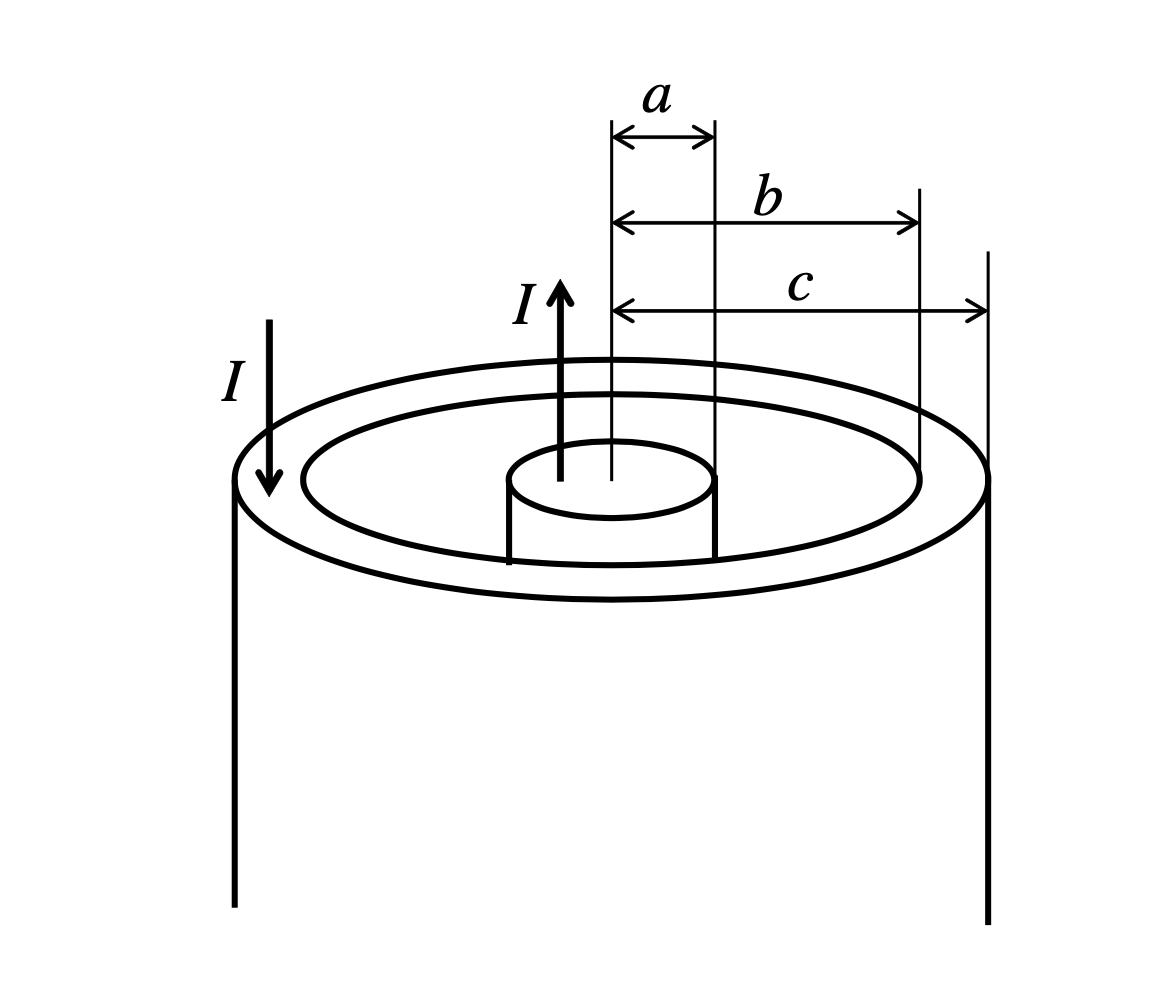
\includegraphics[scale=0.35]{./fig/R03_fig1.png}
	\caption{}
	\label{fig:1}
\end{figure}

\begin{align*}
	r>cのとき&\\
	閉曲面に流れる&電流はI-I=0であるため\\
	H&=0\,[\rm{A/m}]\\
	b<r<cのとき&\\
	dSが上向きである&ことを考慮すると\\
	\int_{C}\boldsymbol{H}\cdot d\boldsymbol{l}&=\int_{C}Hdl=2\pi rH\,[\rm{A}]\\
	\int_{S}\boldsymbol{J}\cdot d\boldsymbol{S}&=\int_{S}JdS=I-\int_{S} \frac{I}{c^{2}\pi-b^{2}\pi}dS\\
	&=I-\frac{I}{c^{2}\pi-b^{2}\pi}\pi(r^{2}-b^{2})=\left(1-\frac{r^{2}-b^{2}}{c^{2}-b^{2}}\right)I\\
	&=\left(\frac{c^{2}-b^{2}-r^{2}+b^{2}}{c^{2}-b^{2}}\right)I=\frac{c^{2}-r^{2}}{c^{2}-b^{2}}I\,[\rm{A}]\\
	2\pi r H&=\frac{c^{2}-r^{2}}{c^{2}-b^{2}}I\\
	H&=\frac{I}{2\pi r}\frac{c^{2}-r^{2}}{c^{2}-b^{2}}\,[\rm{A/m}]\\
	a<r<bのとき&\\
	同様にdSは上向き&とする\\
	\int_{C}\boldsymbol{H}\cdot d\boldsymbol{l}&=\int_{C}Hdl=2\pi rH\,[\rm{A}]\\
	\int_{S}\boldsymbol{J}\cdot d\boldsymbol{S}&=\int_{S} JdS=I\,[\rm{A}]\\
	アンペールの法則より&\\
	H&=\frac{I}{2\pi r}\,[\rm{A/m}]\\
	r<aのとき&\\
	同様にdSは上向き&とする\\
	\int_{C}\boldsymbol{H}\cdot d\boldsymbol{l}&=\int_{C}Hdl=2\pi rH\,[\rm{A}]\\
	\int_{S}\boldsymbol{J}\cdot d\boldsymbol{S}&=\int_{S} JdS=\frac{I}{a^{2}\pi}r^{2}\pi=\frac{r^{2}}{a^{2}}I\,[\rm{A}]\\
	アンペールの法則より&\\
	H&=\frac{\frac{r^{2}}{a^{2}}I}{2\pi r}=\frac{I}{2\pi a^{2}}r\,[\rm{A/m}]\\\\
	\therefore H&=
	\left\{
	\begin{matrix}
	\frac{I}{2\pi a^{2}}r\,[\rm{A/m}] &(0 < r< a)\\\\
	\frac{I}{2\pi r}\,[\rm{A/m}] & (a < r< b) \\\\
	\frac{I}{2\pi r} \frac{c^{2}-r^{2}}{c^{2}-b^{2}}\,[\rm{A/m}] & (b < r <c)\\\\
	0\,[\rm{A/m}] & (r >c)
	\end{matrix}
	\right .  \\
	ただし向きは&左回り(反時計回り)
\end{align*}

\newpage
\section{雨ニモマケズ,風ニモマケズ,\wfig{2}ニ示スヤウナ,単位長サ当タリ$n$巻ノ無限長ソレノイドコイルガアル.コイルニ電流$I$ヲ流シタトキ,コイルノ周囲ニ発生スル磁界$H$ヲアンペールノ法則ヲ用イテ導出スル.サウイフモノニワタシハナリタイ.}

\begin{figure}[h]
	\centering
	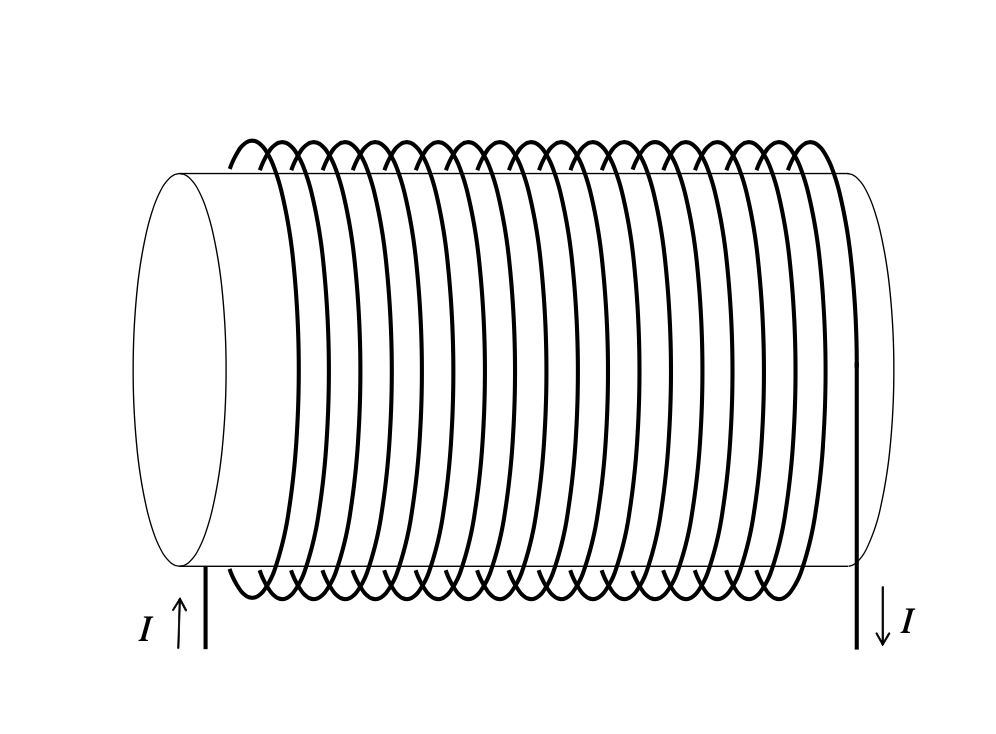
\includegraphics[scale=0.35]{./fig/R03_fig2.png}
	\caption{}
	\label{fig:2}
\end{figure}
\begin{figure}[h]
	\centering
	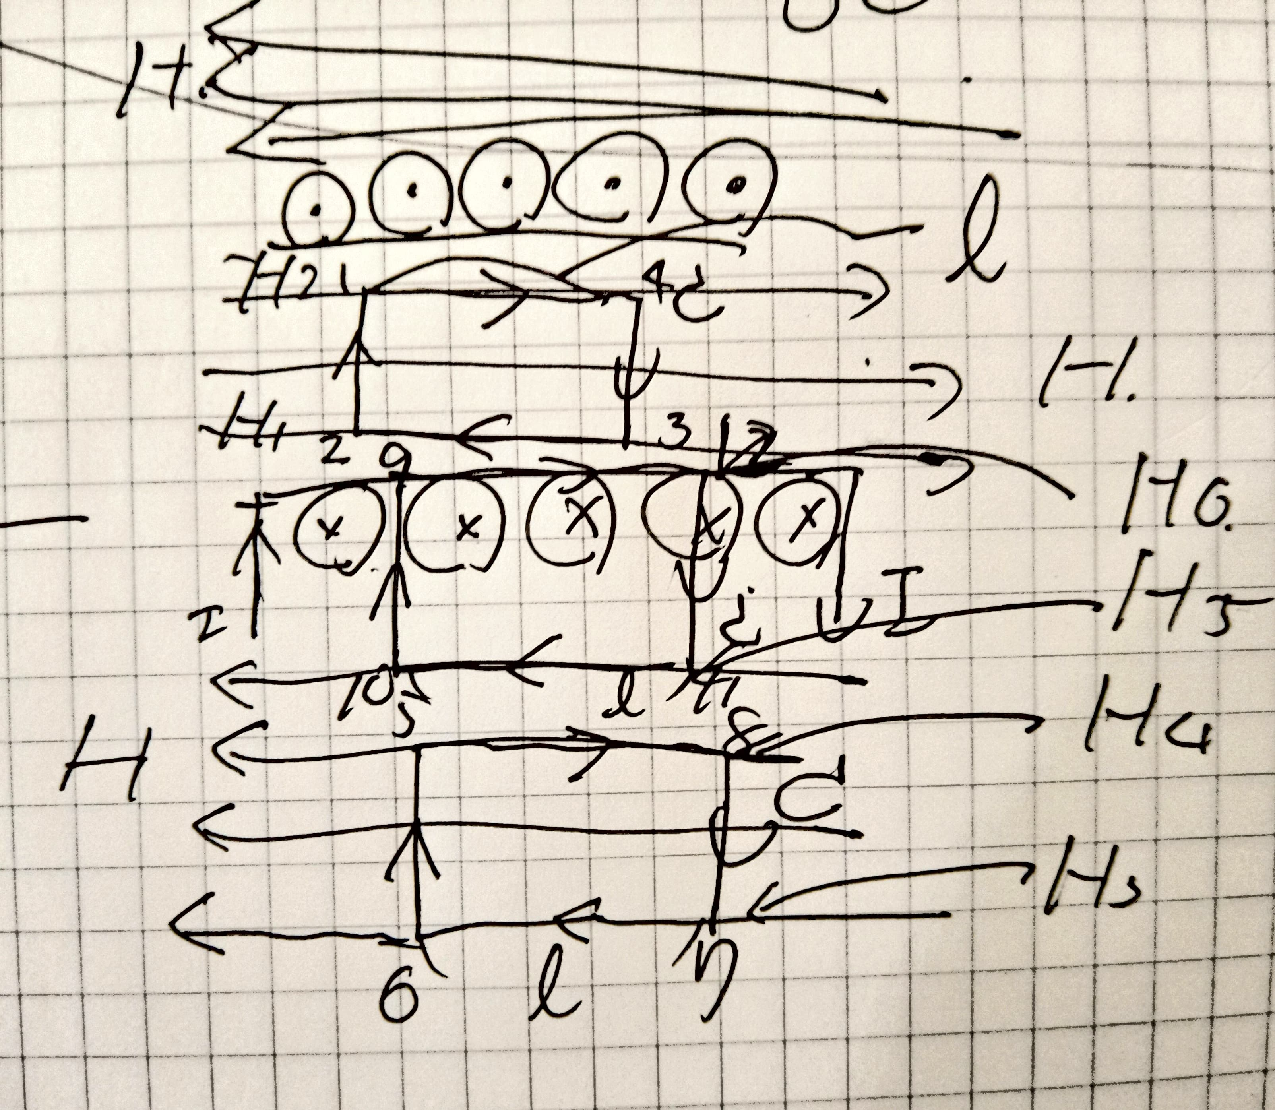
\includegraphics[scale=0.35]{./fig/fig.pdf}
	\caption{}
	\label{fig:a}
\end{figure}


\begin{align*}
このコイルによって発生する磁界はコイル&内部では右向き,コイル外部では左向きとなる.\\
経路Cとしてコイル内に&長方形1234(左上から反時計回りの順)を決める\\
また,経路23上&の磁界をH_{1},経路14上の磁界をH_{2},長さをlとする\\
\int_{C}\boldsymbol{H}\cdot d\boldsymbol{l}&=\int_{12}\boldsymbol{H}\cdot d\boldsymbol{l}+\int_{23}\boldsymbol{H}\cdot d\boldsymbol{l}+\int_{34}\boldsymbol{H}\cdot d\boldsymbol{l}+\int_{41}\boldsymbol{H}\cdot d\boldsymbol{l}\\
\boldsymbol{H}とd\boldsymbol{l}が直交するとき,&内積は0であるため\\
&=\int_{0}^{l}H_{1}dl-\int_{0}^{l}H_{2}dl\\
&=(H_{1}-H_{2})l\,[\rm{A}]\\
\int_{S}\boldsymbol{J}\cdot \boldsymbol{S}&=0\,[\rm{A}]\\
\therefore H_{1}-H_{2}&=0\\
H_{1}&=H_{2}\tag{1}\\
次に経路Cとしてコイル&外部に長方形5678(左上から反時計回りの順)を決める\\
また,経路67上&の磁界をH_{3},経路85上の磁界をH_{4},長さをlとする\\
コイル内の場合と同様の議論により&\\
\int_{C}\boldsymbol{H}\cdot d\boldsymbol{l}&=\int_{56}\boldsymbol{H}\cdot d\boldsymbol{l}+\int_{67}\boldsymbol{H}\cdot d\boldsymbol{l}+\int_{78}\boldsymbol{H}\cdot d\boldsymbol{l}+\int_{85}\boldsymbol{H}\cdot d\boldsymbol{l}\\
\boldsymbol{H}とd\boldsymbol{l}が直交するとき,&内積は0であるため\\
&=-\int_{0}^{l}H_{3}dl+\int_{0}^{l}H_{4}dl\\
&=(H_{4}-H_{3})l\,[\rm{A}]\\
\int_{S}\boldsymbol{J}\cdot \boldsymbol{S}&=0\,[\rm{A}]\\
\therefore H_{4}-H_{3}&=0\\
H_{3}&=H_{4}\\
ここでd \to \infty のときH_{4}&=0\\
\therefore H&=0\,[\rm{A/m}]\left|_{コイル外部}\right .\tag{2}\\
最後に経路Cとしてコイルの境界が経路の中心&となるような長方形9,10,11,12(左上から反時計回りの順)を決める\\
また,経路10,11上&の磁界をH_{5},経路12,9上の磁界をH_{6},長さをlとする\\
今までと同様の議論により&\\
\int_{C}\boldsymbol{H}\cdot d\boldsymbol{l}&=\int_{9,10}\boldsymbol{H}\cdot d\boldsymbol{l}+\int_{10,11}\boldsymbol{H}\cdot d\boldsymbol{l}+\int_{11,12}\boldsymbol{H}\cdot d\boldsymbol{l}+\int_{12,9}\boldsymbol{H}\cdot d\boldsymbol{l}\\
\boldsymbol{H}とd\boldsymbol{l}が直交するとき,&内積は0であり,式(2)よりコイル外部の磁界は0であるため\\
&=H_{5}l\,[\rm{A}]\\
\int_{S}\boldsymbol{J}\cdot \boldsymbol{S}&=\int_{S}JdS=nIl\,[\rm{A}]\\
\therefore H_{5}l&=nIl\\
H_{5}&=nI\,[\rm{A/m}]\\
ここでH_{5}はコイルの内部の磁界であるあるため&式(1)より\\
H&=nI\,[\rm{A/m}]\left|_{コイル内部}\right .
\end{align*}

\newpage
\section{これはこの辺りに住まい致すものにて候.\wfig{3}に示すように,断面積が半径$r$の円で,比透磁率$\mu_{r}$,半径$R$の円環鉄心に導線を$N$巻したコイルが御座ります.このコイルに電流$I$を流したとき,以下に示す各問いに解答頂きたく候.ただし,$r \ll R$ とし,発生した 磁界はすべて鉄心内部に存在し,漏れ磁界は存在致さず候.}
\begin{enumerate}[(a)]
	\item 発生する磁界$H$をアンペールの法則を用いて導出されたく候.
	\begin{align*}
	r&\ll Rであるため\\
	\int_{C}\boldsymbol{H}\cdot d\boldsymbol{l}&=\int_{C}Hdl=2\pi RH\,[\rm{A}]\\
	\int_{S}\boldsymbol{J}\cdot d\boldsymbol{S}&=NI\,[\rm{A}]\\
	\therefore H&=\frac{NI}{2\pi R}\,[\rm{A/m}]
	\end{align*}
	\item 鉄心内部に発生する磁束密度$B$を求められ候.
	\begin{equation*}
	B=\mu H\mu_{0}\mu_{s}H=\frac{\mu_{0}\mu_{s}NI}{2\pi R}\,[\rm{T}]
	\end{equation*}
	\item 鉄心内部に発生する磁束$\Phi$を求められ候.
	\begin{equation*}
	\Phi=BS=\frac{\mu_{0}\mu_{s}NI}{2\pi R}\pi r^{2}=\frac{\mu_{0}\mu_{s}r^{2}NI}{2R}\,[\rm{Wb}]
	\end{equation*}
	\item 起磁力を$NI$とすると磁気抵抗$R_{m}$は$R_{m}=\frac{NI}{\Phi}$で求められるとこによって,この鉄心の磁気抵抗$R_{m}$を求めていただきたくお願い申し上げ候.
	\begin{equation*}
	R_{m}=\frac{NI}{\Phi}=\frac{NI}{\frac{\mu_{0}\mu_{s}r^{2}NI}{2R}}=\frac{2R}{\mu_{0}\mu_{s}r^{2}}\,[\rm{A/Wb}]
	\end{equation*}
\end{enumerate}

\begin{figure}[h]
	\centering
	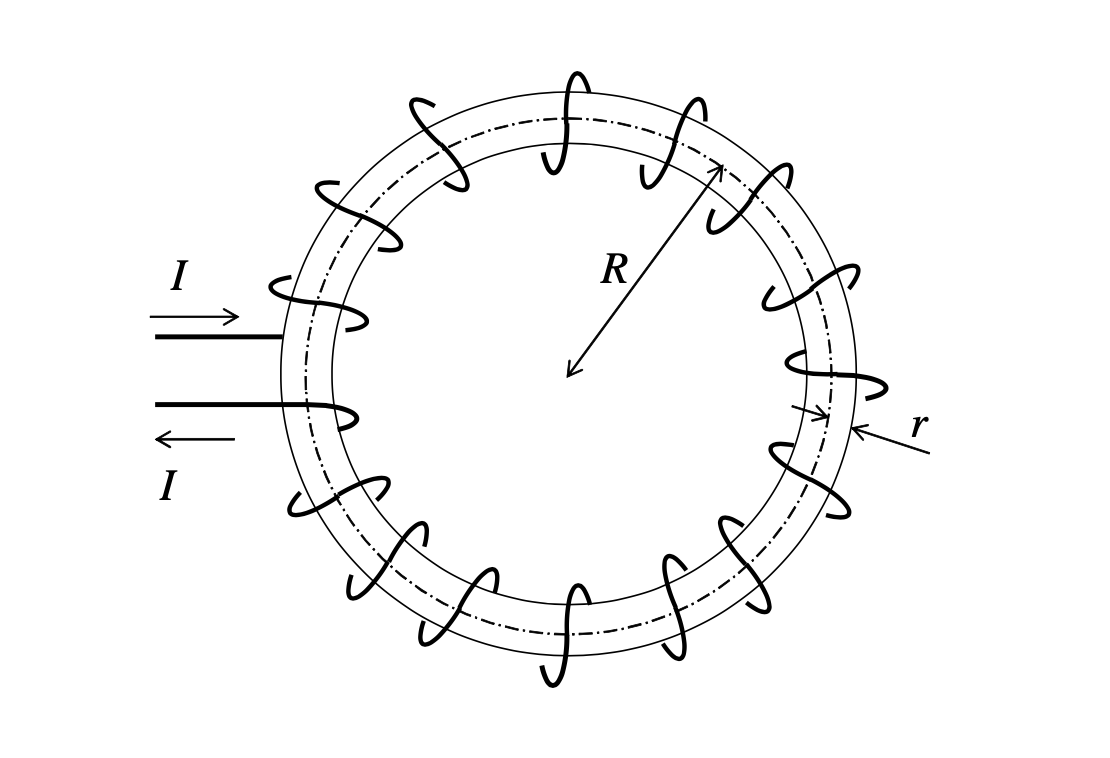
\includegraphics[scale=0.35]{./fig/R03_fig3.png}
	\caption{}
	\label{fig:3}
\end{figure}

\newpage
\section{とざいとうざい.\wfig{4}に示すように,半径$a$の円を断面にもつ無限長円柱導体に中心軸方向の電流密度が流れてさせていただいております.いま,中心からの距離を$r$とし,電流密度$J$が次に示す各場合のとき,導体の内外に発生する磁界$H$を求めて頂きますよう,ひとえにお願い申し上げ奉ります.}
\begin{enumerate}[(a)]
	\item 
	\begin{align*}
	J=
	\left\{
	\begin{matrix}
	J_{1}& (0\leq r \leq a/\sqrt{2})\\
	-J_{1}&(a/\sqrt{2} < r \leq a)
	\end{matrix}
	\right .
	\end{align*}
	ただし,$J_{1}$は正の実定数.
	\item 
	\begin{align*}
	J=\frac{J_{2}}{r}
	\end{align*}
	ただし,$J_{2}$は正の実定数.
\end{enumerate}

\begin{figure}[h]
	\centering
	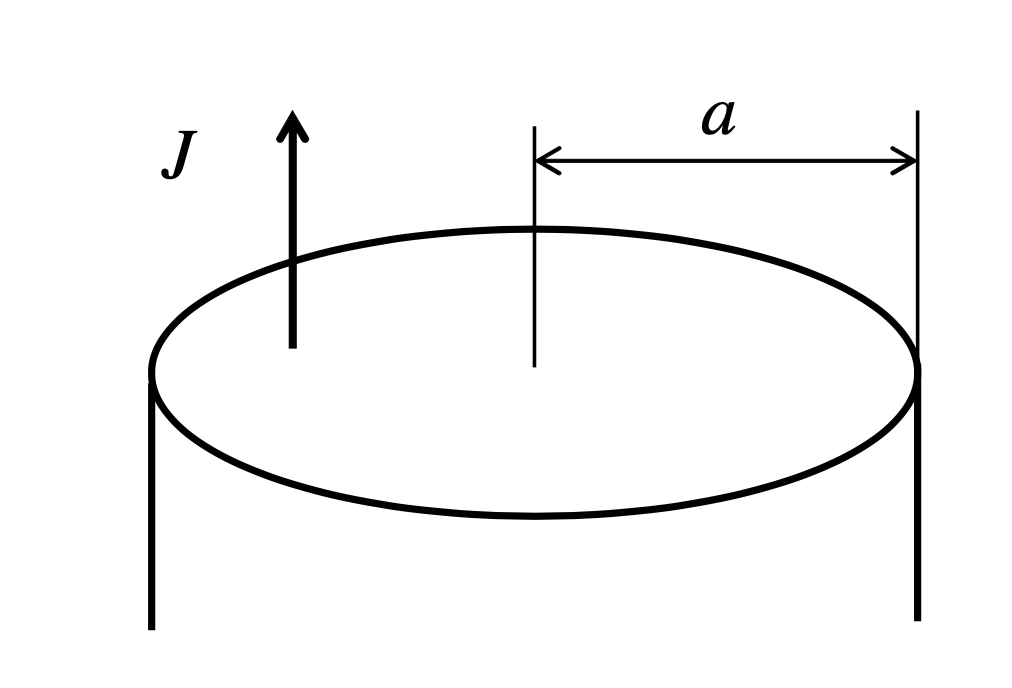
\includegraphics[scale=0.35]{./fig/R03_fig4.png}
	\caption{}
	\label{fig:4}
\end{figure}

\end{document}
